\section{Pregunta N$^{\circ}$2\qquad Khalid Zaid Izquierdo Ayllón}

\begin{frame}
	\frametitle{Método de Newton}
	Dado $F\colon\mathbb{R}^{n}\to\mathbb{R}^{n}$, encuentre
	$x^{\ast}\in\mathbb{R}^{n}$ tal que $F\left(x^{\ast}\right)=0$.
	El \alert{método de Newton} consiste en dado un
	$x^{\left(0\right)}\in\mathbb{R}^{n}$, para $k\geq0$
	hasta alcanzar convergencia resolver el sistema lineal
	\begin{equation*}
		DF
		\left(x^{\left(k\right)}\right)
		h^{\left(k\right)}=
		-F\left(x^{\left(k\right)}\right)
	\end{equation*}
	y actualizar
	\begin{equation*}
		x^{\left(k+1\right)}=
		x^{\left(k\right)}+
		h^{\left(k\right)}.
	\end{equation*}

\end{frame}

\begin{frame}
	\begin{enumerate}\setcounter{enumi}{1}
		\item

		      Resolver el sistema no lineal
		      \begin{math}
			      \left\{
			      \begin{aligned}
				      x^{2} + xy  & = 77 \\
				      xy  + y^{2} & = 44
			      \end{aligned}
			      \right.
		      \end{math}
		      con los métodos de Newton y
		      homotopía.
	\end{enumerate}

	\begin{solution}
		Sean $F\colon\mathbb{R}^{2}\to\mathbb{R}^{2}$ una función suave y
		$DF\left(x,y\right)$ la matriz jacobiana de $F$ en
		$\left(x,y\right)$ dadas por

		\begin{equation*}
			F\left(x,y\right)=
			\begin{bNiceMatrix}
				x^{2} + xy -77 \\
				xy  + y^{2} - 44
			\end{bNiceMatrix},\quad
			DF\left(x,y\right)=
			\begin{bNiceMatrix}
				2x+y & x    \\
				y    & x+2y
			\end{bNiceMatrix}.
		\end{equation*}

		El sistema no lineal $F\left(x\right)=0$ tiene dos soluciones en
		${\left[-20,20\right]}^{2}\subset\mathbb{R}^{2}$.
		Encontremos las soluciones con los métodos pedidos.

		\begin{figure}[ht!]
			\centering
			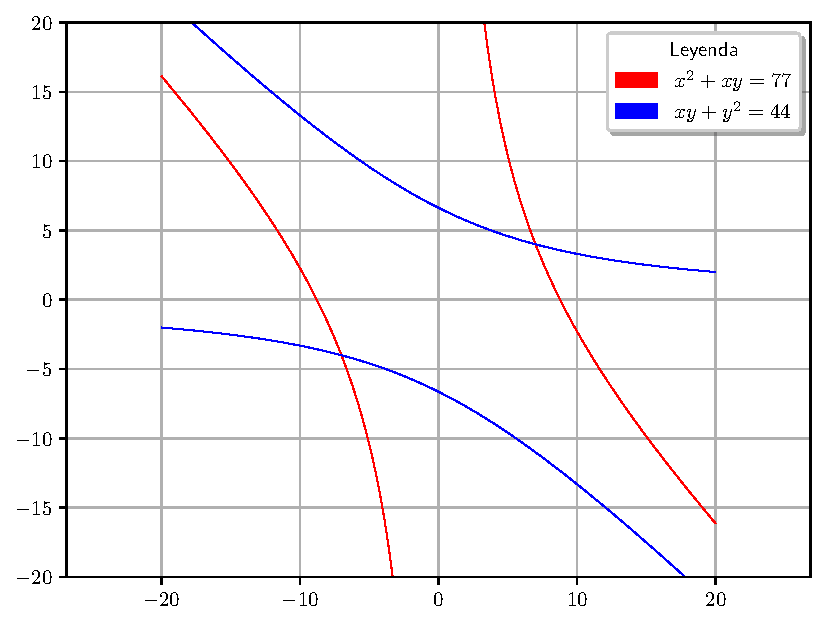
\includegraphics[width=0.45\paperwidth]{p2_plot}
		\end{figure}
	\end{solution}
\end{frame}

\begin{frame}
	\begin{solution}
		\begin{description}
			\item[Método de Newton]

				Sea
				\begin{math}
					x_{0}=
					\begin{bNiceMatrix}
						\alert{1} \\
						\alert{1}
					\end{bNiceMatrix}
				\end{math}
				un punto inicial, una tolerancia $\epsilon=10^{-5}$ y
				$N_{\text{máx}}=10$.
				En la etapa $k=0$, resolver el sistema lineal

				\begin{align*}
					DF
					\left(x^{\left(0\right)}\right)
					h^{\left(0\right)}             & =
					-F\left(x^{\left(0\right)}\right)              \\
					\begin{bNiceMatrix}
						2\times\alert{1}+\alert{1} & \alert{1}                  \\
						\alert{1}                  & \alert{1}+2\times\alert{1}
					\end{bNiceMatrix}
					\begin{bmatrix}
						h_{1}^{\left(0\right)} \\
						h_{2}^{\left(0\right)}
					\end{bmatrix} & =
					-\begin{bNiceMatrix}
						 \alert{1}^{2} + \alert{1}\times\alert{1} -77 \\
						 \alert{1}\times\alert{1}  + \alert{1}^{2} - 44
					 \end{bNiceMatrix} \\
					\begin{bNiceMatrix}
						3 & 1 \\
						1 & 3
					\end{bNiceMatrix}
					\begin{bmatrix}
						h_{1}^{\left(0\right)} \\
						h_{2}^{\left(0\right)}
					\end{bmatrix} & =
					-\begin{bNiceMatrix}
						 -75 \\
						 - 42
					 \end{bNiceMatrix}\xRightarrow{\text{Resolviendo}}
					\begin{bmatrix}
						h_{1}^{\left(0\right)} \\
						h_{2}^{\left(0\right)}
					\end{bmatrix}=
					\begin{bmatrix}
						\dfrac{183}{8} \\
						\dfrac{51}{8}
					\end{bmatrix}.
				\end{align*}
				Y actualizar
				\begin{align*}
					x^{\left(1\right)}\leftarrow
					x^{\left(0\right)}+
					h^{\left(0\right)} \\
					x^{\left(1\right)}=
					\begin{bNiceMatrix}
						1 \\
						1
					\end{bNiceMatrix}+
					\begin{bNiceMatrix}
						\dfrac{183}{8} \\
						\dfrac{51}{8}
					\end{bNiceMatrix}=
					\begin{bNiceMatrix}
						\dfrac{191}{8} \\
						\dfrac{59}{8}
					\end{bNiceMatrix}.
				\end{align*}
				Mientras que $0\leq N_{\text{máx}}$, el
				\begin{math}
					\det
					\left(
					DF\left(x^{\left(0\right)}\right)
					\right)=
					8\geq
					\epsilon
				\end{math}
				y
				\begin{math}
					{\left\|
						x^{\left(1\right)}-
						x^{\left(0\right)}
						\right\|}_{\infty}=
						{\left\|
							h^{\left(0\right)}
							\right\|}_{\infty}=
					\dfrac{183}{8}\geq\epsilon
				\end{math}.
		\end{description}
	\end{solution}
\end{frame}

\begin{frame}
	\begin{solution}
		\begin{description}
			\item[Método de Newton]

				En la etapa $k=1$, resolver el sistema lineal

				\begin{align*}
					DF
					\left(x^{\left(1\right)}\right)
					h^{\left(1\right)}             & =
					-F\left(x^{\left(1\right)}\right)                                                                                                                                              \\
					\begin{bNiceMatrix}
						2\times\alert{\dfrac{191}{8}}+\alert{\dfrac{59}{8}} & \alert{\dfrac{191}{8}}                              \\
						\alert{\dfrac{59}{8}}                               & \alert{\dfrac{191}{8}}+2\times\alert{\dfrac{59}{8}}
					\end{bNiceMatrix}
					\begin{bmatrix}
						h_{1}^{\left(1\right)} \\
						h_{2}^{\left(1\right)}
					\end{bmatrix} & =
					-\begin{bNiceMatrix}
						 {\left(\alert{\dfrac{191}{8}}\right)}^{2} + \alert{\dfrac{191}{8}}\times\alert{\dfrac{59}{8}} -77 \\
						 \alert{\dfrac{191}{8}}\times\alert{\dfrac{59}{8}}  + {\left(\alert{\dfrac{59}{8}}\right)}^{2} - 44
					 \end{bNiceMatrix} \\
					\begin{bNiceMatrix}
						\dfrac{441}{8} & \dfrac{191}{8} \\
						\dfrac{59}{8}  & \dfrac{309}{8}
					\end{bNiceMatrix}
					\begin{bmatrix}
						h_{1}^{\left(1\right)} \\
						h_{2}^{\left(1\right)}
					\end{bmatrix} & =
					-\begin{bNiceMatrix}
						 -\dfrac{21411}{32} \\
						 -\dfrac{5967}{32}
					 \end{bNiceMatrix}\xRightarrow{\text{Resolviendo}}
					\begin{bmatrix}
						h_{1}^{\left(1\right)} \\
						h_{2}^{\left(1\right)}
					\end{bmatrix}=
					\begin{bmatrix}
						-\dfrac{2738151}{250000} \\
						-\dfrac{684099}{250000}
					\end{bmatrix}.
				\end{align*}
				Y actualizar
				\begin{align*}
					x^{\left(2\right)}\leftarrow
					x^{\left(1\right)}+
					h^{\left(1\right)} \\
					x^{\left(2\right)}=
					\begin{bNiceMatrix}
						\dfrac{191}{8} \\
						\dfrac{59}{8}
					\end{bNiceMatrix}+
					\begin{bNiceMatrix}
						-\dfrac{2738151}{250000} \\
						-\dfrac{684099}{250000}
					\end{bNiceMatrix}=
					\begin{bNiceMatrix}
						\dfrac{3230599}{250000} \\
						\dfrac{1159651}{250000}
					\end{bNiceMatrix}.
				\end{align*}
				Mientras que $0\leq N_{\text{máx}}$, el
				\begin{math}
					\det
					\left(
					DF\left(x^{\left(1\right)}\right)
					\right)=
					\dfrac{15625}{8}\geq
					\epsilon
				\end{math}
				y
				\begin{math}
					{\left\|
						x^{\left(2\right)}-
						x^{\left(1\right)}
						\right\|}_{\infty}=
						{\left\|
							h^{\left(1\right)}
							\right\|}_{\infty}=
					\dfrac{2738151}{250000}\geq\epsilon
				\end{math}.
		\end{description}
	\end{solution}
\end{frame}

% \begin{frame}
% 	\begin{solution}
% 		De manera análoga, con el punto inicial
% 		$x_{0}=\left(-1,-1\right)$, se obtendrá la otra solución.
% 	\end{solution}
% \end{frame}

\begin{frame}[fragile]
	\begin{columns}
		\begin{column}{0.48\textwidth}
			\inputminted[fontsize=\tiny,firstline=1,lastline=21]{python}{p2_newton.py}
			\inputminted[fontsize=\tiny,firstline=58,lastline=60]{python}{p2_newton.py}
		\end{column}
		\begin{column}{0.48\textwidth}
			\inputminted[fontsize=\tiny,firstline=23,lastline=55]{python}{p2_newton.py}
		\end{column}
	\end{columns}
\end{frame}

\begin{frame}[fragile]
	Para
	\begin{math}
		x_{0}=
		\begin{bNiceMatrix}
			1 \\
			1
		\end{bNiceMatrix}
	\end{math}.
	\begin{center}
		\begin{minipage}{0.5\textwidth}
			\inputminted[fontsize=\tiny,firstline=1,lastline=17]{text}{resultado_pregunta_2.txt}
		\end{minipage}
	\end{center}

	Para
	\begin{math}
		x_{0}=
		\begin{bNiceMatrix}
			-1 \\
			-1
		\end{bNiceMatrix}
	\end{math}.
	\begin{center}
		\begin{minipage}{0.5\textwidth}
			\inputminted[fontsize=\tiny,firstline=18,lastline=35]{text}{resultado_pregunta_2.txt}
		\end{minipage}
	\end{center}
\end{frame}

\begin{frame}
	\begin{solution}
		\begin{description}
			\item[Método de Homotopía]
                    Sea
				\begin{math}
					x_{0}=
					\begin{bNiceMatrix}
						\alert{-5} \\
						\alert{-5}
					\end{bNiceMatrix}
				\end{math}
				un punto inicial, un
				$N_{\text{máx}}=10$ y un $h=0.10$

                Para $K1=h(-J(W_0)^-1$

				.
 		\end{description}
	\end{solution}
 \end{frame}